\documentclass[11pt,a4paper]{article}
\usepackage[utf8]{inputenc}
\usepackage[T1]{fontenc}
\usepackage{lmodern}
\usepackage[margin=1in]{geometry}
\usepackage{amsmath}
\usepackage{listings}
\usepackage{xcolor}
\usepackage{graphicx}
\usepackage{caption}
\usepackage{subcaption}
\usepackage{float}
\usepackage{pgfplots}
\pgfplotsset{compat=1.17}

\lstset{
  keywordstyle=\bfseries,
  showstringspaces=false,
  breaklines=false,
  language=C,
  morekeywords={size_t},
  literate=
    {**}{{$\ast\mskip-3mu\ast$}}2
    {*}{{$\ast$}}1
    {-}{{$-$}}1,
}

\title{HPP Assignment 4: Report}
\author{Lukas Billera, Filip Helgsten, Anton von Nandelstadh}
\date{}

\begin{document}
\maketitle

\section{The Problem}
This assignment extends the galaxy simulation from Assignment 3 with parallelism using
Pthreads and OpenMP. The computational bottleneck is the $O(N^2)$ pairwise force computation,
which is where we devote our parallelization efforts.

\section{The Solution}
Profiling the serial baseline code showed that the pairwise force loop accounts for around 99.9\%
of the runtime for our problem sizes (e.g., 8.187s out of 8.191s for $N = 5000$).

The Pthreads version creates \texttt{n\_threads} worker threads and assigns the outer loop with a
cyclic distribution (\texttt{n = id; n < N; n += nthreads}). Each thread accumulates acceleration
contributions in \texttt{axnup}/\texttt{aynup} arrays of length $N$. After each timestep there is a barrier and
thread 0 reduces these contributions into the global acceleration arrays, updates velocity and
position, resets the temporary arrays, and then a second barrier releases the workers for the
next timestep.

\begin{lstlisting}[caption={Pthreads Parallelization}]
typedef struct {
    int id;
    int nthreads;
    int nsteps;
    double dt;
    int N;
    double* px;
    double* py;
    double* mass;
    double* vx;
    double* vy;
    double* axn;
    double* ayn;
    double** axnup;
    double** aynup;
    pthread_barrier_t *pbarr;
} GalParams;

void* pairloop(void* args) {
    GalParams params = *(GalParams*)(args);
    int N = params.N;
    double* axnup = params.axnup[params.id];
    double* aynup = params.aynup[params.id];
    for (int time = 0; time < params.nsteps; time++) {
        for (int n = params.id; n < N; n+=params.nthreads) {
            double px_n = params.px[n];
            double mass_n = params.mass[n];
            double py_n = params.py[n];
            double axn = 0, ayn = 0;
            for (int m = n + 1; m < N; m++) {
                double xdiff = px_n-params.px[m];
                double ydiff = py_n-params.py[m];
                double e0 = 0.001;
                double G = 100 / (double)N;
                double r = sqrt(xdiff * xdiff + ydiff * ydiff) + e0;
                double r3 = r * r * r;
                double force_x = -G * xdiff / r3;
                double force_y = -G * ydiff / r3;
                axn += params.mass[m] * force_x;
                ayn += params.mass[m] * force_y;
                axnup[m] -= mass_n * force_x;
                aynup[m] -= mass_n * force_y;
            }
            axnup[n] += axn;
            aynup[n] += ayn;
        }
        pthread_barrier_wait(params.pbarr);
        if (params.id == 0) {
            for (int n=0;n<N;n++){
                for (int k=0; k<params.nthreads; k++) {
                    params.axn[n] += params.axnup[k][n];
                    params.ayn[n] += params.aynup[k][n];
                }
            }
            for (int n =0; n<N; n++) {
                params.vx[n] += params.dt*params.axn[n];
                params.vy[n] += params.dt*params.ayn[n];
                params.px[n] += params.dt*params.vx[n];
                params.py[n] += params.dt*params.vy[n];
            }
            for (int k =0; k< params.nthreads; k++) {
                memset(params.axnup[k], 0, params.N*sizeof(double));
                memset(params.aynup[k], 0, params.N*sizeof(double));
            }
            memset(params.axn, 0, params.N*sizeof(double));
            memset(params.ayn, 0, params.N*sizeof(double));
        }
        pthread_barrier_wait(params.pbarr);
    }
    return NULL;
}
\end{lstlisting}

The OpenMP version uses the same pairwise algorithm and the same idea of per-thread
temporary arrays, but replaces the explicit thread management with \texttt{\#pragma omp parallel}
and \texttt{\#pragma omp for schedule(dynamic)} on the outer loop. The dynamic schedule was
chosen because of the load imbalance in the outer-loop and as in the pthreads version we use a
single thread for the other parts of the program.

\begin{lstlisting}[basicstyle=\small,keywordstyle=\mdseries,language=,xleftmargin=1em]
#pragma omp parallel num_threads(nthreads)
{
int id = omp_get_thread_num();
for (int time = 0; time < nsteps; time++) {
    #pragma omp for schedule(dynamic)
    for (int n = 0; n < N; n++) {
        double px_n = px[n];
        double mass_n = mass[n];
        double py_n = py[n];
        double axn = 0, ayn = 0;
        for (int m = n + 1; m < N; m++) {
            double xdiff = px_n-px[m];
            double ydiff = py_n-py[m];
            double e0 = 0.001;
            double G = 100 / (double)N;
            double r = sqrt(xdiff * xdiff + ydiff * ydiff) + e0;
            double r3 = r * r * r;
            double force_x = -G * xdiff / r3;
            double force_y = -G * ydiff / r3;
            axn += mass[m] * force_x;
            ayn += mass[m] * force_y;
            axnup[id][m] -= mass_n * force_x;
            aynup[id][m] -= mass_n * force_y;
        }
        axnup[id][n] += axn;
        aynup[id][n] += ayn;
    }
    #pragma omp single
    {
        for (int n=0;n<N;n++){
            for(int k=0; k<nthreads; k++) {
                ax[n] += axnup[k][n];
                ay[n] += aynup[k][n];
            }
        }
        for (int n =0; n<N; n++) {
            vx[n] += dt*ax[n];
            vy[n] += dt*ay[n];
            px[n] += dt*vx[n];
            py[n] += dt*vy[n];
        }
        for (int k =0; k< nthreads; k++) {
            memset(axnup[k], 0, N*sizeof(double));
            memset(aynup[k], 0, N*sizeof(double));
        }
        memset(ax, 0, N*sizeof(double));
        memset(ay, 0, N*sizeof(double));
    }
}
}
\end{lstlisting}

Other parallelization options were considered but not used. For example, we initially implemented the pthreads parallelization by creating and joining threads in the pairwise force loop,
but the overhead of creating threads was very large. This led us to pursuing this path where
the threads are created only once and we have tried to solve the load balance concerns by either
using cyclic distribution of work in Pthreads or simply using dynamic for openmp.

\section{Performance and Discussion}
All timings were on an Intel(R) Core(TM) Ultra 9 275HX. For \texttt{best\_timing.txt}, five runs
were made at 24 threads and the minimum observed time was reported.

\begin{figure}[H]
\centering
\begin{subfigure}[b]{0.48\textwidth}
\centering
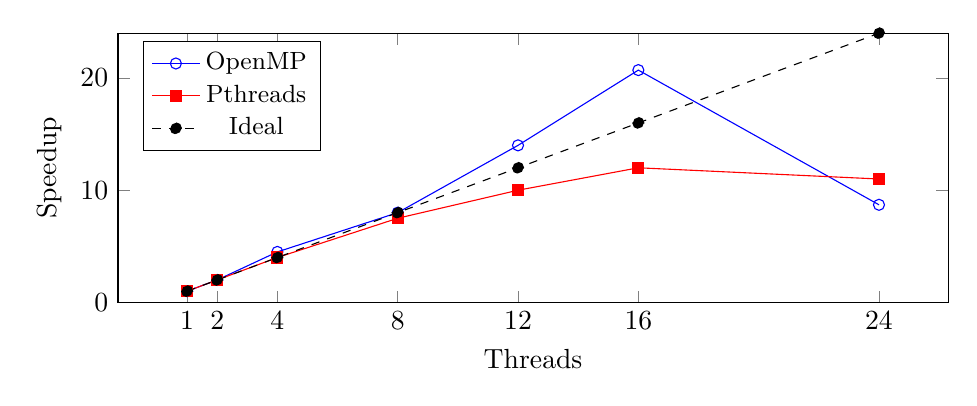
\begin{tikzpicture}
\begin{axis}[
    width=\textwidth,
    height=5cm,
    xlabel={Threads},
    ylabel={Speedup},
    xtick={1,2,4,8,12,16,24},
    ymin=0, ymax=24,
    legend pos=north west,
    legend style={font=\small},
]
\addplot[blue, mark=o] coordinates {(1,1) (2,2) (4,4.5) (8,8) (12,14) (16,20.71) (24,8.70)};
\addlegendentry{OpenMP}
\addplot[red, mark=square*] coordinates {(1,1) (2,2) (4,4) (8,7.5) (12,10) (16,12) (24,11)};
\addlegendentry{Pthreads}
\addplot[black, dashed, mark=*] coordinates {(1,1) (2,2) (4,4) (8,8) (12,12) (16,16) (24,24)};
\addlegendentry{Ideal}
\end{axis}
\end{tikzpicture}
\caption{$N = 2000$}
\end{subfigure}
\hfill
\begin{subfigure}[b]{0.48\textwidth}
\centering
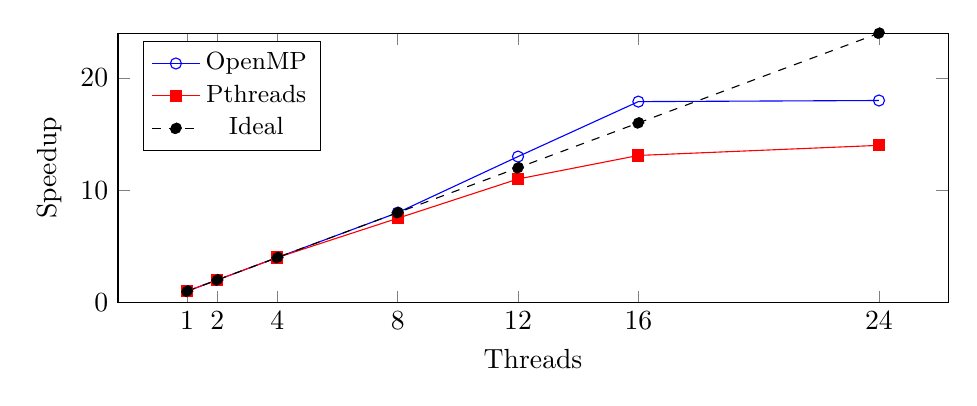
\begin{tikzpicture}
\begin{axis}[
    width=\textwidth,
    height=5cm,
    xlabel={Threads},
    ylabel={Speedup},
    xtick={1,2,4,8,12,16,24},
    ymin=0, ymax=24,
    legend pos=north west,
    legend style={font=\small},
]
\addplot[blue, mark=o] coordinates {(1,1) (2,2) (4,4) (8,8) (12,13) (16,17.9) (24,18)};
\addlegendentry{OpenMP}
\addplot[red, mark=square*] coordinates {(1,1) (2,2) (4,4) (8,7.5) (12,11) (16,13.1) (24,14)};
\addlegendentry{Pthreads}
\addplot[black, dashed, mark=*] coordinates {(1,1) (2,2) (4,4) (8,8) (12,12) (16,16) (24,24)};
\addlegendentry{Ideal}
\end{axis}
\end{tikzpicture}
\caption{$N = 5000$}
\end{subfigure}
\end{figure}

For $N = 2000$, OpenMP scaled very well up to 16 threads, where it reached a speedup of
20.71, but dropped sharply at 24 threads to 8.70.

For $N = 5000$, both versions scaled more consistently. OpenMP no longer had a sharp drop
at 24 threads and both achieved relatively good scaling performance at 16 threads (17.9 and
13.1 at 16 threads). They again struggled to do much better with 24 threads.

The best times were 0.413131s for Pthreads and 0.390458s for OpenMP on \texttt{ellipse\_N\_05000.gal}
with 100 timesteps, $\Delta t = 10^{-5}$.

\section{AI disclosure}
AI (chatGPT, claude) was used for help with debugging, e.g. why does this code segfault, and
was also used to help visualizing runtimes above.

\end{document}
